\section{Mô tả tính năng của phần mềm}
Đồ án Game Cờ vua 2 người cung cấp một phần mềm mô phỏng môn thể thao trí tuệ Cờ vua, với tính năng 2 người chơi. Phần mềm cung cấp đầy đủ các tính năng cơ bản của một game cờ vua như các bước di chuyển, tính năng bắt quân, chiếu, phong cấp cho quân Tốt, nhập thành...\\
Phần mềm được thiết kế và xây dựng trên nền tảng Linux (Ubuntu 20.04), vì vậy, những tính năng sau đây cũng được ví dụ trên nền tảng này.

\subsection{Màn hình khởi động của game}
Hình sau đây là màn hình khởi động của game, với đầy đủ các quân cờ đã được sắp xếp vào vị trí, sẵn sàng cho một trận chiến mới.
\begin{figure}[H]
\centering{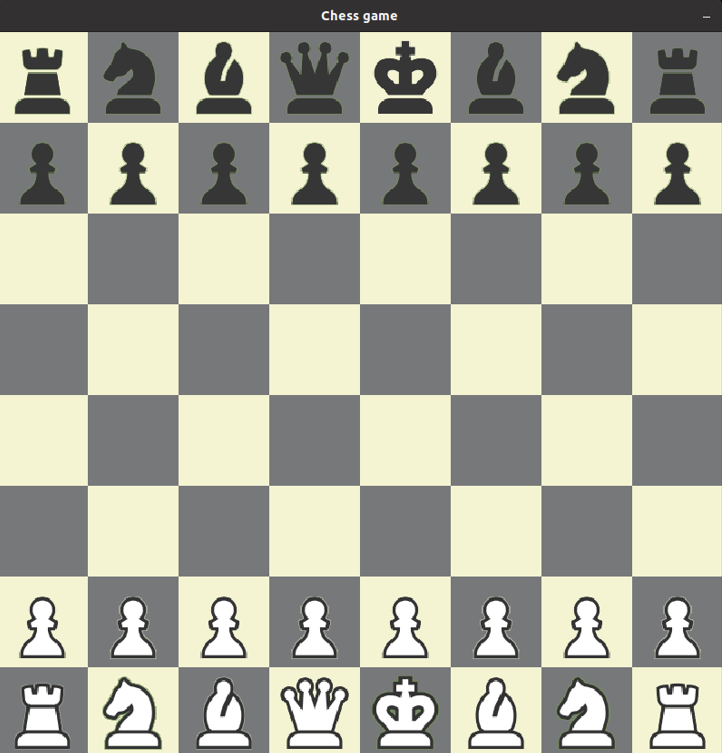
\includegraphics[scale=0.5]{images/features/Start}}
\caption{Màn hình khởi động của game}
\end{figure}

\subsection{Di chuyển quân cờ}
Hình sau đây là nước đi đầu tiên trong game, với quân Tốt trắng tiến lên hai bước.
\begin{figure}[H]
\centering{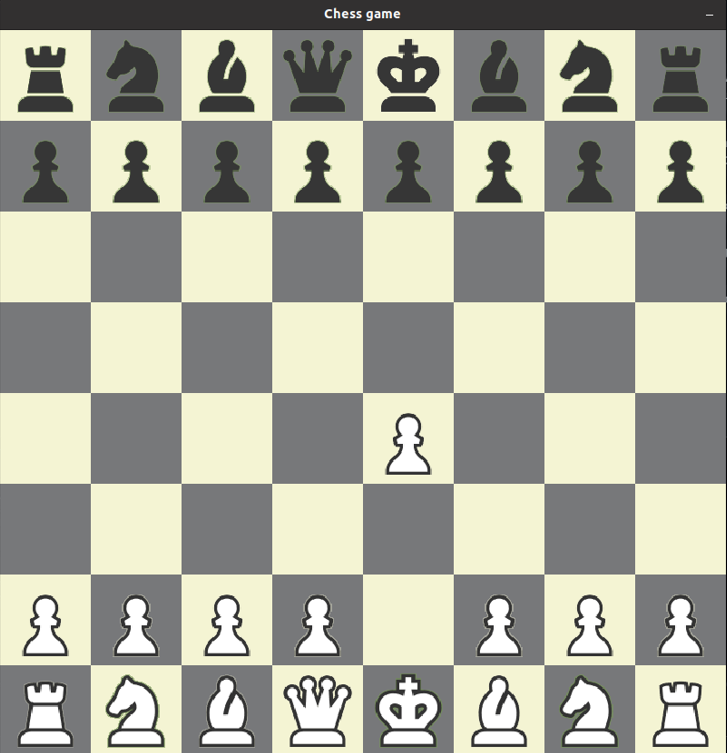
\includegraphics[scale=0.5]{images/features/FirstMove}}
\caption{Di chuyển quân cờ trong game}
\end{figure}

\subsection{Tính năng bắt (ăn) quân}
Hình sau đây là ví dụ về tính năng bắt quân theo đường chéo của quân Tốt trắng đối với quân Tốt đen, sau khi quân Tốt đen này tiến vào ô có thể bị bắt bởi quân Tốt trắng. Quân cờ bị bắt sẽ bị loại khỏi bàn chơi ngay lập tức.
\begin{figure}[H]
\centering{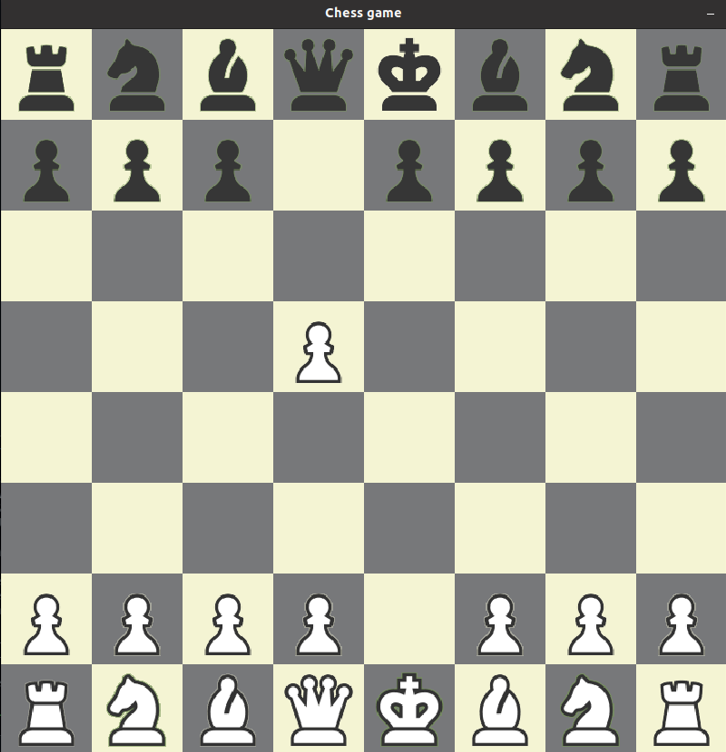
\includegraphics[scale=0.5]{images/features/Capture}}
\caption{Bắt quân cờ của đối thủ}
\end{figure}

\subsection{Chiếu}
Hình sau đây mô tả tình huống quân Vua bị chiếu, tức là quân Vua nằm trong một ô có thể bị bắt ở các quân cờ của đối thủ. Ô bị chiếu hiện tại sẽ được tô màu đỏ. Sau khi bị chiếu, quân Vua phải di chuyển đến nơi an toàn, hoặc những quân cờ khác phải di chuyển để "cắt" đường chiếu của quân cờ đối thủ, thậm chí có thể bắt quân cờ này để bảo vệ vua. Nếu không thể, ván đấu sẽ kết thúc và bên bị chiếu sẽ thua cuộc.
\begin{figure}[H]
\centering{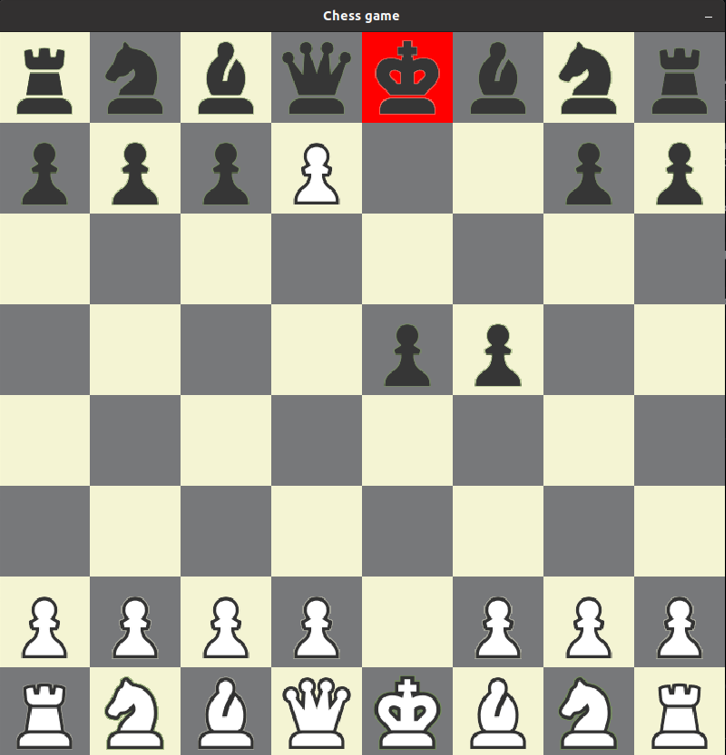
\includegraphics[scale=0.5]{images/features/Check}}
\caption{Chiếu}
\end{figure}

\subsection{Thăng cấp (Phong cấp) cho quân Tốt}
Khi quân Tốt tiến đến hàng cuối cùng trên "địa phận" của đối thủ, nó sẽ được thăng cấp thành một trong bốn quân: Hậu, Xe, Tượng, Mã. Hình sau đây mô tả một ví dụ về tính năng thăng cấp cho quân Tốt này.
\begin{figure}[H]
\centering{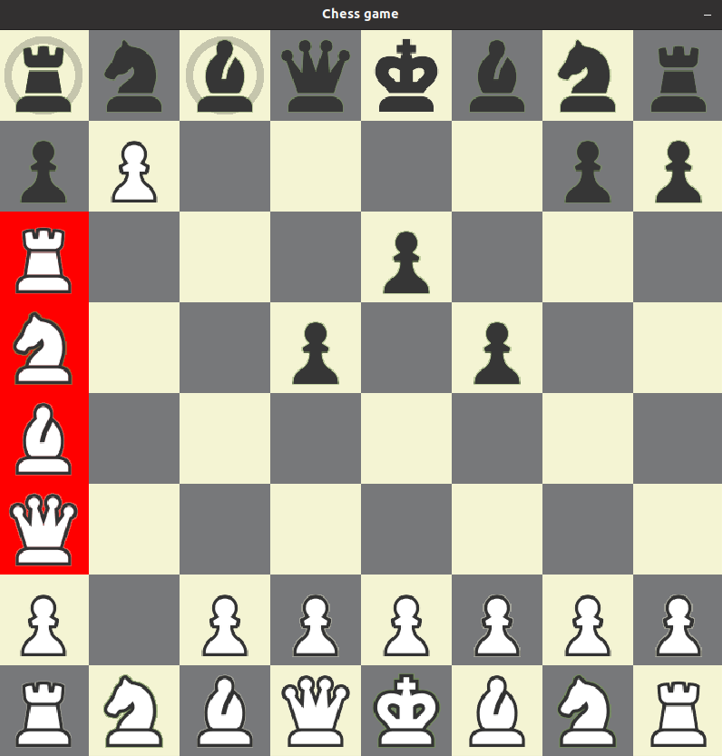
\includegraphics[scale=0.5]{images/features/Promote}}
\caption{Thăng cấp cho quân Tốt}
\end{figure}

\subsection{Nhập thành}
Khi quân Vua và quân Xe của một bên chưa di chuyển, các ô giữa chúng đều trở thành ô trống và ô đích đến không bị chiếu thì quân Vua có thể tiến hành nhập thành. Có hai loại nhập thành, ứng với hai quân Xe, lần lượt là long castling (tạm dịch là "nhập thành dài") $-$ ứng với quân Xe ở xa Vua hơn và short castling (tạm dịch là "nhập thành ngắn) $-$ ứng với quân Xe ở gần Vua hơn. Hình sau đây cho ta một ví dụ về nhập thành dài.
\begin{figure}[H]
\centering{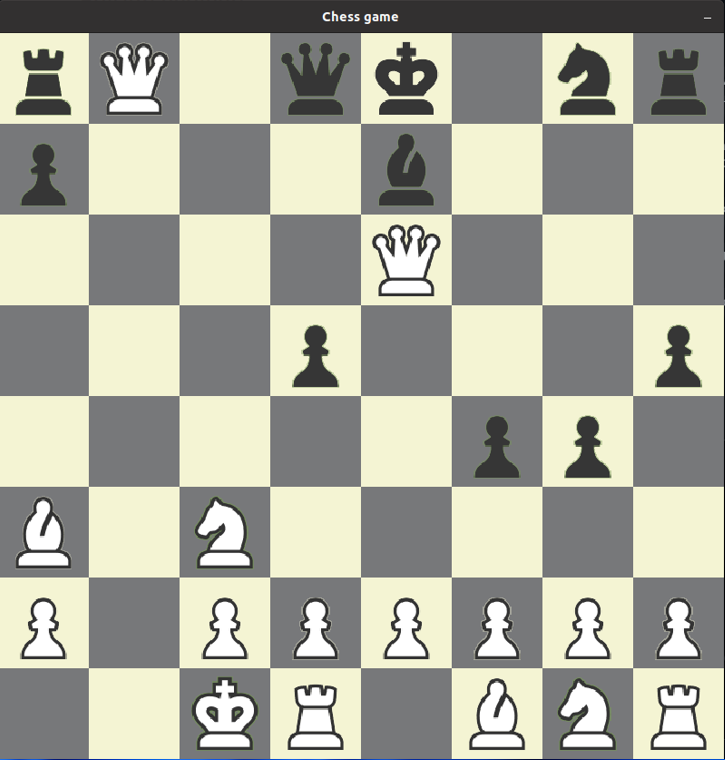
\includegraphics[scale=0.5]{images/features/Castling}}
\caption{Nhập thành}
\end{figure}

\subsection{Kết thúc ván đấu (chiếu hết)}
Khi quân Vua bị chiếu và không còn nước đi nào khác có thể "cứu" quân Vua ra khỏi ô bị chiếu này, ván đấu sẽ kết thúc với chiến thắng cho bên chiếu. Hình sau đây cho ta một ví dụ về bàn cờ lúc kết thúc ván đấu.
\begin{figure}[H]
\centering{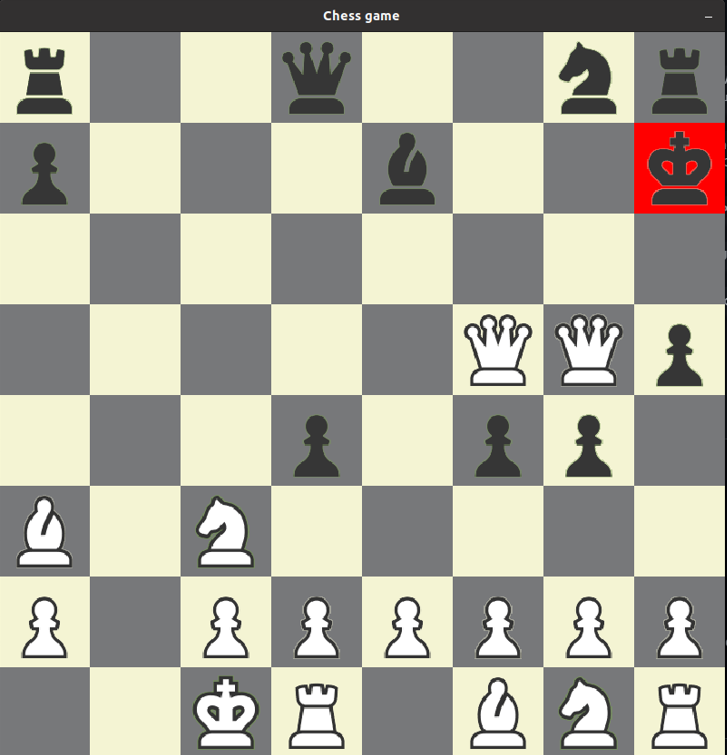
\includegraphics[scale=0.5]{images/features/Checkmate}}
\caption{Kết thúc ván đấu (chiếu hết)}
\end{figure}
Khi tình huống này xảy ra, một thông báo sẽ hiện lên màn hình console, cho ta biết người chiến thắng.
\begin{figure}[H]
\centering{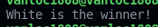
\includegraphics[scale=3]{images/features/Winner}}
\caption{Thông báo người chiến thắng}
\end{figure}

\subsection{Thoát game}
Ta có thể thoát game bằng cách tắt cửa sổ game hoặc nhấn phím Escape (Esc) ở góc trên bên trái bàn phím.